% !TEX root = ../../main.tex

\section{Handling state changes} % (fold)
\label{sec:handling_state_changes}

\subsection{InstantSearch}
\label{ssec:instantsearch}

The InstantSearch state container is exposed as a factory function creating a new container. The {\tt createInstantSearch} function inherits from the {\tt createStore} function used in other parts of the \gls{library}, see figure \ref{figure:createstore_inheritance} for the complete architecture. It allows to be subscribed to with a function as argument that will be called each time a change happens to the state, with the new state as arguments.

While all three keys of the state container will change over time, they each work in a slightly different way. The {\tt results} key is described in section \ref{sec:getting_responses_from_the_api}, and is tracked fairly straightforward. Every time a new \acrshort{api} response comes in, it will completely overwrite the previous state of that key.

\begin{figure}[H]
  \centering
  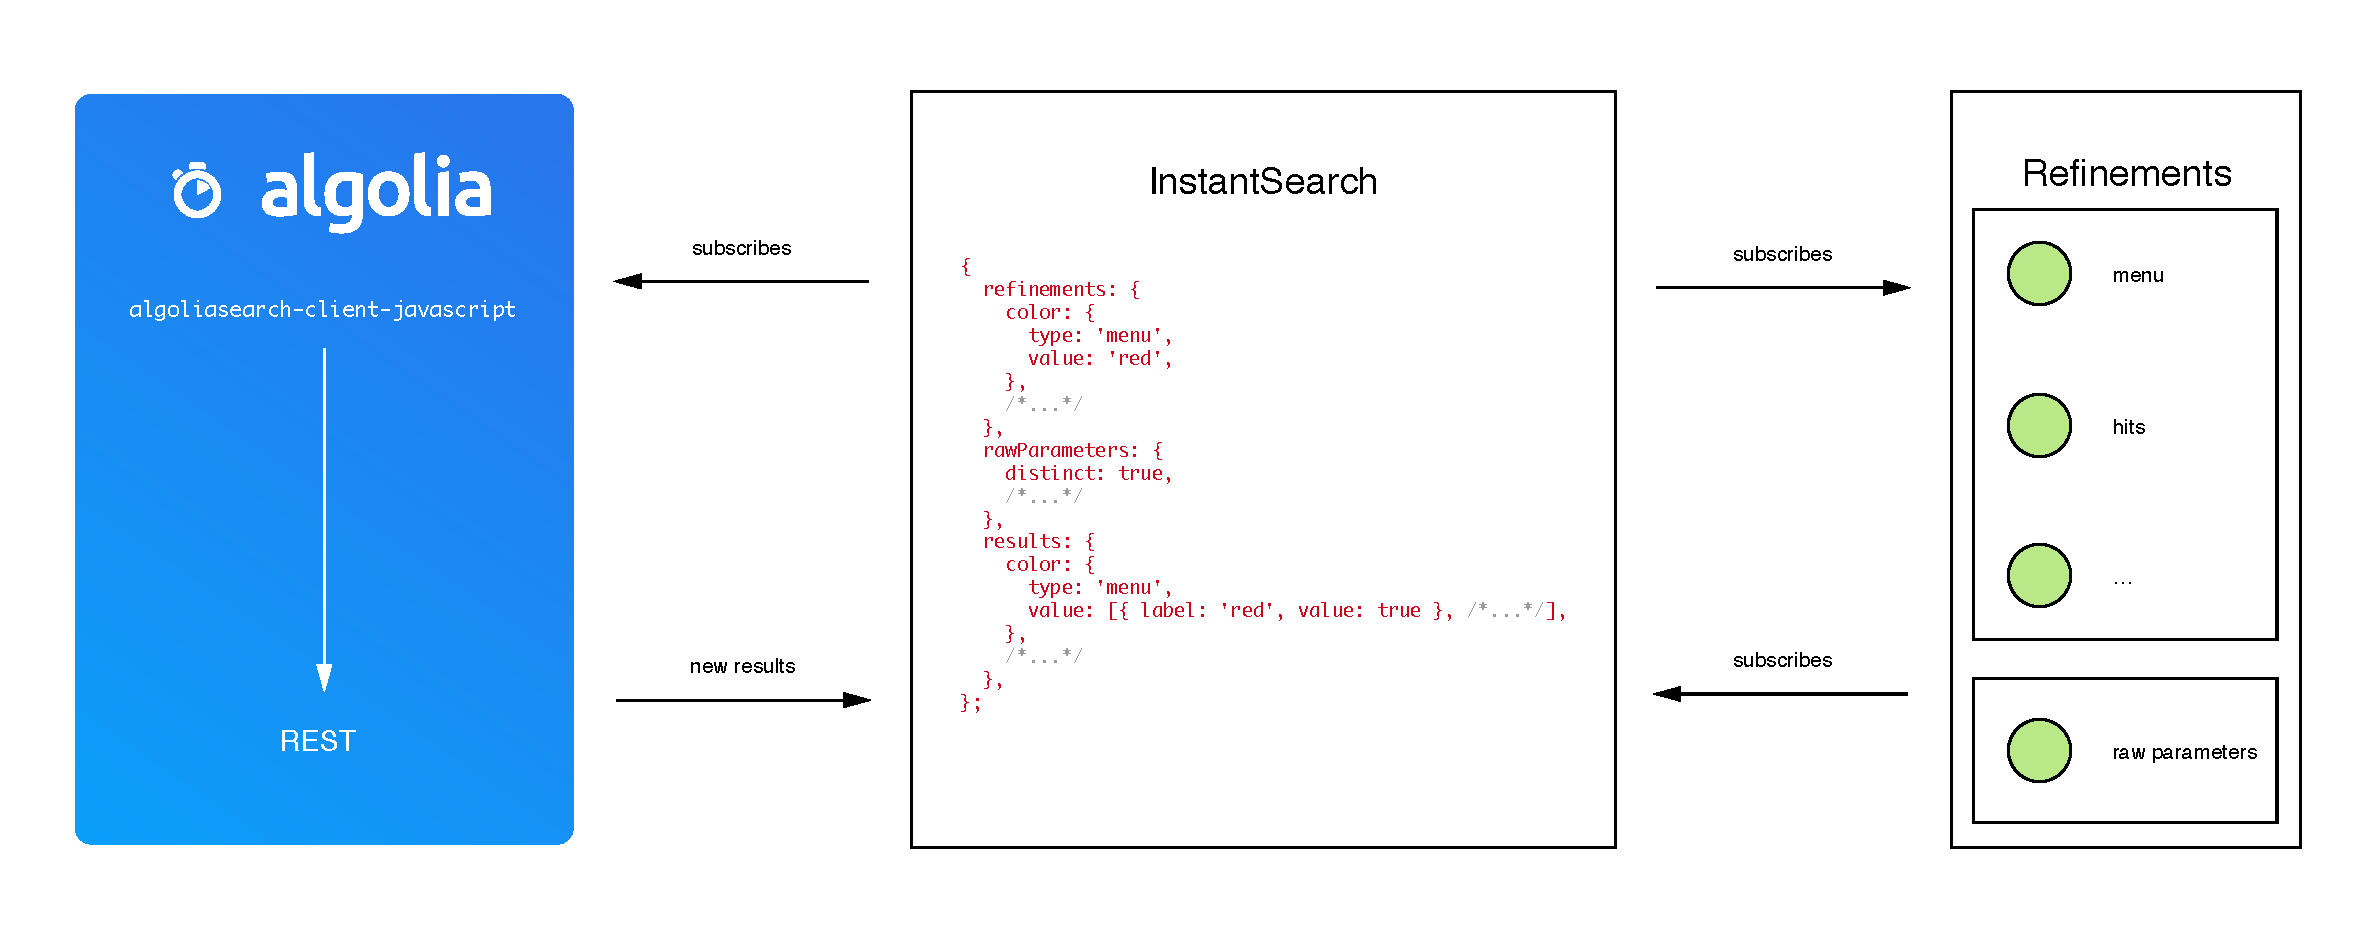
\includegraphics[width=\textwidth]{../assets/is-core-architecture.pdf}
  \caption{Architecture overview}
  \label{figure:core-architecture}
\end{figure}

\subsection{Raw \glspl{refinement}}
\label{ssec:raw-refinments}

All raw parameters are being rewritten in place, similar to how {\tt setState} works in React~\cite{react-doc-state}~. A function called {\tt refineRaw} is exposed on a state container. This function expects a function as an argument. It receives the previous state for the \glspl{refinement} as its parameter, and is expected to return the new state Object, based on whatever happened that needs to change.

This pattern allows a developer to have the freedom to change whatever parameters are necessary to change, while having access to the complete truth at that point easily. An example of toggling the {\tt DISTINCT} parameter, for example on an event listener for a button with that purpose would look like this:

\begin{minipage}{\linewidth}
\begin{lstlisting}[caption={Toggling the {\tt DISTINCT} parameter},label={lst:is-core-raw}]
function toggleDistinct(previousState) {
  // set the distinct parameter as the opposite of previously
  const oppositeDistinct = { distinct: !previousState.distinct };

  // make an Object to hold the new state
  const newState = Object.assign({}, previousState, oppositeDistinct);
  return newState;
}

state.refineRaw(toggleDistinct);
\end{lstlisting}
\end{minipage}

In future JavaScript engines\footnote{spread properties on Objects are currently a Stage 3 proposal for \acrshort{ecmascript}\cite{es-prop-spread}, which means they are starting to be implemented by browsers, but it isn't part of the standard yet.}, it will be able to write this kind of code using spread properties on Objects. This kind of pattern would look like this then:

\begin{minipage}{\linewidth}
\begin{lstlisting}[caption={Toggling the {\tt DISTINCT} parameter when Object spread is available},label={lst:is-core-raw-es2015}]
function toggleDistinct(previousState) {
  return {
    ...previousState,
    distinct: distinct: !previousState.distinct,
  }
}

state.refineRaw(toggleDistinct);
\end{lstlisting}
\end{minipage}

\subsection{Refinements}
\label{ssec:refinments}

The complete state container is structured in the same way as a single refinement. It's a factory function, returning an Object. This Object has three functions: 

\begin{enumerate}
  \item {\tt get state()}
  \item {\tt subscribe()}
  \item {\tt setState()} or {\tt refine()}
\end{enumerate}

A basic {\tt store} will call all of the subscribers with the new state, as soon as {\tt setState} is being called. This simple subscriber pattern allows one store to work the same for the main state container, as well as for refinements. In refinements, the {\tt setState} function is being renamed to {\tt refine}, because this is the terminology used by other InstantSearch flavours, and fits well with the name of a {\tt refinement}.

\begin{figure}[H]
  \centering
  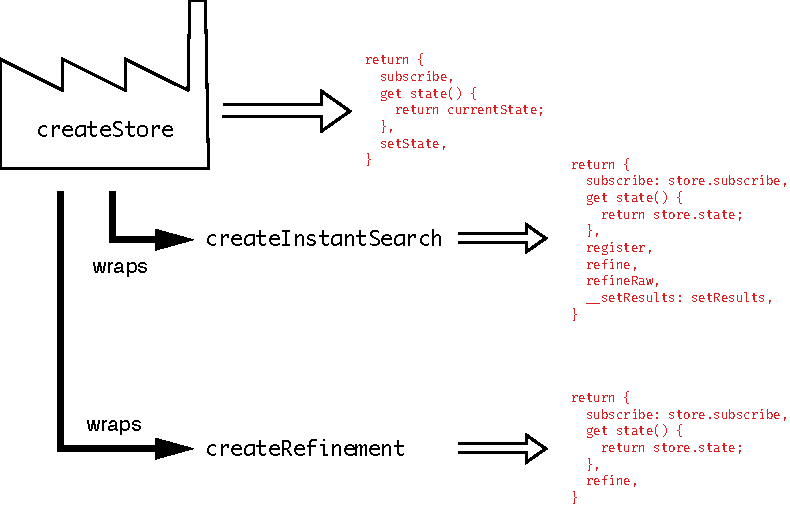
\includegraphics[width=\textwidth]{../assets/create-store.pdf}
  \caption{InstantSearch Core store organisation.}
  \label{figure:createstore_inheritance}
\end{figure}

\subsection{Subscribing}
\label{ssec:Subscribing}

The big differentiator between some of the big frontend frameworks nowadays is how they handle state changes. To make sure that InstantSearch Core to be used in all major methodologies, three different interfaces are exposed.

\subsubsection{Getters}
\label{ssub:getters}

While at any moment it's possible to call the state getter on an InstantSearch store or a refinement, a programmer might want to know how state changes overtime, and get notified about the new change. If only the state getter would be implemented, a naive way to find out about changes, is repeatedly asking for the current state like this:

\begin{minipage}{\linewidth}
\begin{lstlisting}[caption={Naive way to find out about changed state},label={lst:is-core-naive-subscribe}]
// holder for the state
let currentState = {};

function update() {
  // reassign the state
  currentState = store.state;
  requestAnimationFrame(update);
}

// call the update function when a new frame is being drawn
requestAnimationFrame(update);
\end{lstlisting}
\end{minipage}

After that, the {\tt currentState} variable might be used wherever it's needed, and make the needed UI changes. Depending on the type of framework used for this, it might either have a very big impact, or be optimised away, but it isn't always ideal.

For a framework like Vue\cite{vue-reactivity}, this approach is close to the way to go. There is no implicit need for reassigning a local variable, since the {\tt store} is available with a getter. Vue will track the changes to all getters on Objects with a process called ``reactive values''.

Vue will trigger a new render on every frame where there has been time for it, which gives it the time to call a getter function on every frame seamlessly. 

\subsubsection{Subscribe function}
\label{ssub:subscribe_function}

Not all frameworks implement this kind of reactivity. React for example will only look at the \gls{props} and context of a component. It would be possible to pass down the {\tt store.state} getter as part of React context, but it would cause unneeded renders, since that part of optimisation is left over to the user land of a React app. 

For frameworks like React, a {\tt subscribe()} function is available at the store prototype. Similar to Redux\cite{redux-glossary-store}, a state management \gls{library} that works very well with React, this function expects a single function as the argument. This function will be called at every time the state changes, be it either by changing \glspl{refinement}, or by new results being returned.

This data can then either be passed through as a global variable, via props or via a context, which is an abstraction over props that aren't visible to the user.

To allow unsubscription from a refinement or store, the return value of {\tt .subscribe} is its own cleanup function, which in that case simply has to be called during the cleanup phase.

\subsubsection{Observables}
\label{ssub:observables}

An upcoming proposed standard for \acrshort{ecmascript} is observables.The \acrshort{ecmascript} proposal for Observables is currently stage 0\cite{tc39-observable}, that means that it will not be part of JavaScript until it has been voted for, and went through the process. It's currently not implemented in any browser without libraries. These Observables signify a variable that will change over time, and that will let its subscribers know about the changes.

This pattern is very close to previous method, subscriptions, but then as part of the language, and not a decided upon standard. Using language features has the advantage that over time more libraries will use this pattern and it will make the \acrshort{api} surface of the \gls{library} smaller.

Since the observables implementation in JavaScript is a proposal, a reference implementation has been made by zenparsing, the author of the proposal. The \gls{library} called {\tt zen-observable}\cite{zenparsing-observable} is extending the \acrshort{api} of the Observable proposal slightly, but in its core, it has the same concepts.

An instance of an Observable is returned from the store interface, by using the {\tt symbol-observable}\cite{symbol-observable} ponyfill module. A ponyfill\cite{ponyfill} is a module with the functionality of an upcoming language \acrshort{api}, made with the current capabilities of the platform. The difference between a polyfill and a ponyfill is that a polyfill will overwrite the implementation of the \acrshort{api} if it is implemented in browsers, while a ponyfill intentionally uses a slightly different name.

Just like in the previous section, an Observable will expose a subscribe function. The difference here is that it expects to be subscribed with an Object. This Object contains three functions, that are called when respectively the {\tt next}, {\tt error} or {\tt complete} event have been called by the observable.

Having a interoperability layer with observables means that InstantSearch means that it will work well with the frameworks that use observables as a core of their infrastructure. Angular is an example of a framework that has observables --- in the form of RxJS\cite{angular-rx} --- as an important part of its way to work with events.

% section handling_state_changes (end)
